\vspace{3cm}
\begin{center}
\section{Лекция 3. Выпуклые множества}
\end{center}
\subsection{Полупространства. Гиперплоскости}

\textbf{Определение 2.9}\\
Для $a\in\mathbb{R}^n\setminus \left \{ \mathbb{O}_n \right \}$ и $\beta\in\mathbb{R}$ множества
\begin{center}
\textbf{$H^\leq(a,\beta):= \left \{ x\in\mathbb{R}^n: \left \langle a,x \right \rangle \leq \beta \right \}$} \\
\end{center}
и
\begin{center}
\textbf{$H^=(a,\beta):= \left \{ x\in\mathbb{R}^n: \left \langle a,x \right \rangle = \beta \right \}$} \\
\end{center}
называют определёнными $(a,\beta)$ (афинным) полупространством и (афинной) гиперплоскостью соответственно. (В случае $\beta=0$: линейными).\\

\noindent\textbf{Замечание 2.10}
\begin{itemize}
    \item Полупространства являются выпуклыми и замкнутыми.
\end{itemize}
\begin{itemize}
    \item Гиперплоскости являются выпуклыми.
\end{itemize}
\begin{itemize}
    \item Афинные подпространства являются выпуклыми.
\end{itemize}
\begin{itemize}
    \item Пересечение любого количества полупространств является выпуклым.
\end{itemize}
\subsection{Полиэдры (многогранники)}
\textbf{Определение 2.11}\\
Подмножество $P\subseteq \mathbb{R}^n$ называют (выпуклым) полиэдром, если $P$ является пересечением конечного количества афинных полупространств.
\begin{itemize}
    \item $P = \varnothing$ и $P = \mathbb{R}^n$ (пересечение по пустому индексному множеству) являются полиэдрами.
\end{itemize}
\begin{itemize}
    \item Афинные подпространства являются полиэдрами.
\end{itemize}
\textbf{Замечание 2.12}
\begin{itemize}
    \item Полиэдры являются выпуклыми и (топологически) замкнутыми.
\end{itemize}
\begin{itemize}
    \item Множество допустимых решений (допустимое множество)
\begin{center}
\textbf{$P^\leq(A,b):= \left \{ x\in\mathbb{R}^n:  Ax  \leq b \right \}$}\\
\end{center}
задачи линейной оптимизации является полиэдром.
\end{itemize}

\newpage
\subsection{Полиэдры: примеры}
\begin{figure}[h!]
\centering
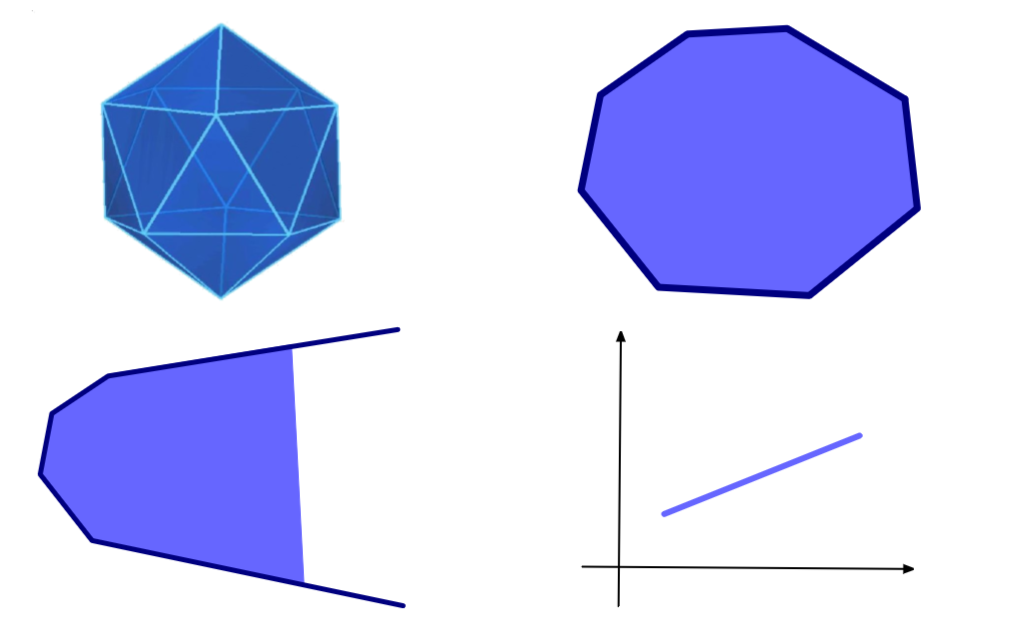
\includegraphics[width=0.9\textwidth]{800px-Polyeder}
\label{fig:}
\end{figure}

\subsection{Суммы Минковского и масштабирование}
\textbf{Определение 2.13}\\
Для множеств $X_1,\ldots,X_q\subseteq \mathbb{R}^n$ выражение
\begin{center}
\textbf{$\sum^{q}_{i=1}{X_i} = X_1+\ldots+X_q := \left\{ \sum^{q}_{i=1}{x^{(i)}}: x^{(i)}\in X_i, \forall i \in [q] \right\}$}\\
\end{center}
называют суммой Минковского множеств $X_1,\ldots,X_q$.\\

\noindent\textbf{Замечание 2.14}\\
Суммы Минковского и масштабирование выпуклых множеств являются выпуклыми множествами.\\
\textbf{$X\subseteq \mathbb{R}^n, \alpha \in \mathbb{R}: \alpha X:= \left\{ \alpha x \mid x \in X \right\}$} ~--- масштабирование множества $X$.

\subsection{Теоремы отделимости для выпуклых множеств}
\textbf{Терема 2.15 (Теорема о разделяющей гиперплоскости)}\\
Пусть $X\subseteq \mathbb{R}^n$ является выпуклым и замкнутым и  $y\in \mathbb{R}^n \setminus X$, тогда существуют такие $a\in\mathbb{R}^n\setminus\left\{\mathbb{O}_n\right\}$ и $\varepsilon>0$, что \textbf{$\left \langle a,x \right \rangle \leq \left \langle a,y \right \rangle - \varepsilon$} для $\forall x\in X$.\\

\noindent$\blacktriangleleft$ Сделаем допущение, что $X\neq\varnothing$. $\varnothing$ замкнуто и выпукло, но для него теорема очевидно выполняется, т.~к. $\forall x \in \varnothing$.\\
Итак, $X\neq \varnothing$. Выберем $a\in\mathbb{R}^n\setminus \left \{ \mathbb{O}_n \right \}$, $\varepsilon>0$\\

\begin{figure}[h!]
\centering
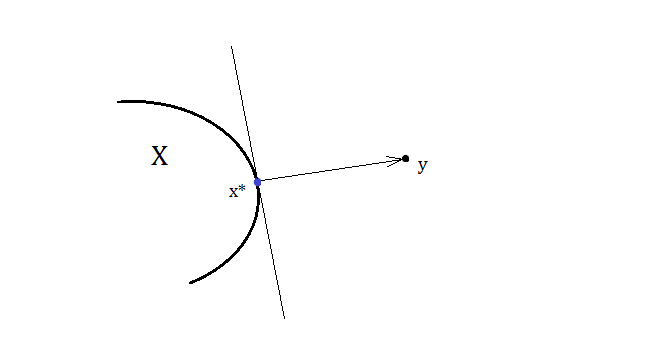
\includegraphics[width=0.9\textwidth]{800px-Beweis1}
\label{fig:}
\end{figure}

\noindent Будем строить гиперплоскость. Покажем, что существует минимум расстояния от y до X (обозначим его $x^{\ast}$). Для этого важно свойство замкнутости. Если бы $X$ было ограниченным, то $X$ было бы компактом. Пересечём $X$, если оно не ограничено, с шаром большего радиуса ~--- получим компакт.\\

\noindent Пусть $x^{\ast} \in X$ такой, что $\parallel y - x^{\ast} \parallel = \min \left\{\parallel y - x \parallel : x \in X \right\}$. Причём, $x^{\ast}$ существует, т.~к., если выбрать $\bar{x}\in X \neq \varnothing$,\\
$\bar{X}:=\left\{ x\in X: \parallel y-x \parallel \leq \parallel y - \bar{x} \right\}$\\
$\inf \left\{ \parallel y - x\parallel : x\in X \right\} = \inf \left\{ \parallel y - x\parallel : x\in \bar{X} \right\}$ $(\ast)$\\
функция $x\longmapsto \parallel y - x\parallel$ ~--- непрерывна, $\bar{X}$ ~--- компакт, и эта функция принимает значения инфимумов $(\ast)$.\\

\noindent Определим: $a = y - x^{\ast}$ и $\varepsilon = \parallel a \parallel ^2$.\\
Покажем, что выбор $a$ и $\varepsilon$ корректен.\\
Предположим, что $\exists x\in X \mid \langle a,x\rangle > \langle a,y \rangle - \varepsilon $ $(\ast\ast)$, причём $ \langle a,y \rangle - \varepsilon = \langle a,y \rangle - \langle a,a \rangle = \langle a,y-a \rangle = \langle a,x^{\ast} \rangle$.\\
Покажем, что этого не может быть.\\

\begin{figure}[h!]
\centering
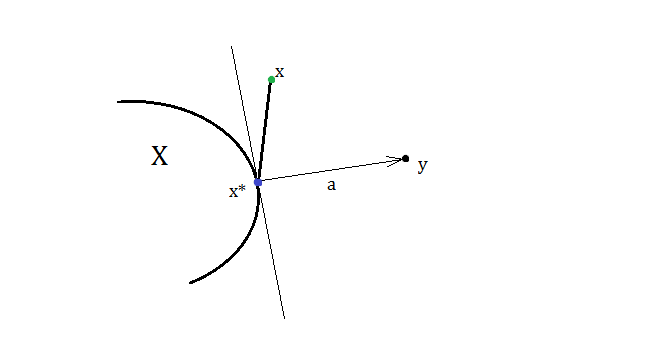
\includegraphics[width=0.9\textwidth]{800px-Beweis2}
\label{fig:}
\end{figure}

\noindent Противоречие:\\

\noindent По соединяющему $x^{\ast}$ и $x$ отрезку точки должны иметь меньшее расстояние до $y$.\\
Посмотрим, что происходит с расстоянием от $y$ до точек прямой при движении в направлении $x$.\\

\noindent Определим функцию $\phi : \mathbb{R} \rightarrow \mathbb{R} $, где  $\phi (t):= \parallel y-(x^{\ast} +t(x-x^{\ast}))\parallel ^2$, причём $x^{\ast} +t(x-x^{\ast}) = (1-t)x^{\ast}+tx$.\\
Достаточно показать, что $\phi ^\prime (0)<0$ потому, что если производная $<0$, то $\exists 0<\tilde{t}\leq 1$ такое, что $\phi (0)>\phi (\tilde{t}) = \parallel y- \tilde{x} \parallel ^2$, где $\tilde{x} = x^{\ast} + \tilde{t}(x-x^{\ast}) \in X$, т.~к. $X$ ~-- выпуклое, а $\phi (0)=\parallel y-x^{\ast} \parallel ^2$. А это противоречие с минимальностью $x^{\ast}$.\\

\noindent$\phi ^\prime (t) = \frac{\textit{d}}{\textit{d}x} \langle y-(x^{\ast}+t(x-x^{\ast})),y-(x^{\ast}+t(x-x^{\ast}))\rangle = \frac{\textit{d}}{\textit{d}x} (\langle y-x^{\ast} \rangle ^{2} - 2 \langle y-x^{\ast},x-x^{\ast}\rangle t + \langle x-x^{\ast}\rangle ^{2} t^{2}) = -2\langle y-x^{\ast},x-x^{\ast}\rangle + 2 \langle x-x^{\ast}\rangle^{2} t$ \\

\noindent $\phi^\prime (0) = -2 \langle y-x^{\ast},x-x^{\ast}\rangle = 2 \langle a,x-x^{\ast}\rangle = 2 (\langle a,x^{\ast}\rangle - \langle a,x\rangle) < 0$,\\
т.~к. из $(\ast\ast)$ вытекает, что $\langle a,x^{\ast}\rangle < \langle a,x\rangle $. $\blacktriangleright$\\

\noindent\textbf{Лемма 2.16a}\\
Пусть $X\subseteq \mathbb{R}^n$ ~-- выпуклое, $y \in \mathbb{R}^{n} \setminus X$. Тогда существует $a \in \mathbb{R}^{n} \setminus \left\lbrace\mathbb{O}\right\rbrace$ что $\left\langle a,x \right\rangle \leq \left\langle a,y \right\rangle \text{, } \forall x \in X$\\
$\blacktriangleleft$
\begin{itemize}
\item Достаточно построить последовательность $y^{(k)} \in \mathbb{R}^{n} \setminus cl(X)$, чтобы $\lim_{k \rightarrow \infty} y^{(k)} =y$.
\begin{itemize}
\item  По теореме 2.15 (т.к. $cl(X)$ замкнуто и выпукло) существует  $a^{(k)} \in \mathbb{R}^{n} \setminus \left\lbrace \mathbb{O} \right\rbrace$, что  $\left\langle a^{(k)},x \right\rangle \leq \left\langle a^{(k)},y^{(k)} \right\rangle \text{, } \forall k \in \mathbb{N} \text{, } \forall x \in cl(X)$
\item С помощью масштабирования сделаем $\| a^{(k)}\| =1 \text{, } \forall k \in \mathbb{N}$, по Теореме Больцано-Вейерштрасса существует $K \subseteq \mathbb{N}$ что $\lim a^{(k)}=a \in \mathbb{R}^{n} \text{, при } k \rightarrow \infty \text{, } k \in K$
\item Т.к. $\| a^{(k)}\| =1$ и $\| \text{ } \|$ - непрерывное отображение, то $\| a\| =1 \text{ и } \Longrightarrow a \neq \mathbb{O} $
\item Имеем $\forall x \in X$:
\begin{itemize}
\item  $\left\langle a^{(k)},x \right\rangle \leq \left\langle a^{(k)},y^{(k)} \right\rangle \text{, } \forall k \in \mathbb{N}$
\item Т.к. скалярное произвендение непрерывно $\Longrightarrow \text{ } \left\langle a,x \right\rangle \leq \left\langle a,y \right\rangle$
\end{itemize}
\end{itemize}
\item Существование последовательности $y^{(k)} \in \mathbb{R}^{n} \setminus cl(X) \text{, что } \lim_{k \rightarrow \infty} y^{(k)}=y$ следует из того, что для $k \in \left\lbrace 1,2,\text{...}\right\rbrace$ не все точки
    \begin{equation*}
    v^{(0)}:=y -\frac{1}{k}\mathbbm{1} \text{, } v^{(1)}:=y +\frac{1}{k}\mathbbm{e_{1}} \text{, } v^{(n)}:=y +\frac{1}{k}\mathbbm{e_{n}}
    \end{equation*}
    лежат в $cl(X)$.
\begin{itemize}
\item Предположим, что $v^{(0)}\text{, }v^{(1)}\text{, ...,}v^{(n)} \in cl(X)$, тогда $\displaystyle y=\sum_{i=1}^{n}\frac{1}{n+1}v{(i)} \in int(cl(X)) \subseteq X$. Противоречие, т.к. $y \notin X$. $\blacktriangleright$
\end{itemize}
\end{itemize}

\noindent\textbf{Терема 2.16}\\
Пусть $X, Y\subseteq \mathbb{R}^n$ ~--- выпуклые множества и $X \cap Y = \varnothing$. Тогда существует такой $a\in\mathbb{R}^n\setminus \left \{ \mathbb{O}_n \right \}$, что \textbf{$\left \langle a,x \right \rangle \leq \left \langle a,y \right \rangle$} для $\forall x\in X, y \in Y$.\\
$\blacktriangleleft$
\begin{itemize}
\item Множества $X,Y \in \mathbb{R}^{n}$ -выпуклы и $X\cap Y = \varnothing$
\item Множество $X + \left( (-1) Y\right):=X-Y$ - выпукло (т.к. сумма Минковского выпуклых множеств является выпуклым множеством) и $\mathbb{O} \notin X-Y$
\item Из Леммы 2.16a $\Longrightarrow \text{ } \exists \text{ } a \in \mathbb{R}^{n} \setminus \left\lbrace \mathbb{O} \right\rbrace \text{ :} \left\langle a, x-y \right\rangle \leq \left\langle a, \mathbb{O}  \right\rangle \text{ ,} \forall x \in X \text{ ,} \forall y \in Y$.
\item Т.к. $ \left\langle a, \mathbb{O}  \right\rangle = 0$, то  $\left\langle a, x-y \right\rangle \leq \left\langle a, \mathbb{O}  \right\rangle \text{ } \Longleftrightarrow \left \langle a,x \right \rangle \leq \left \langle a,y \right \rangle$. $\blacktriangleright$
\end{itemize}
\subsection{Топологическое замыкание}
\textbf{Замечание 2.17}\\
Для любого выпуклого множества $X \subseteq \mathbb{R}^n$ его топологическое замыкание  $cl(X)$ также является выпуклым.\\

\noindent\textbf{Следствие 2.18}\\
Топологическое замыкание любого выпуклого множества есть пересечение всех содержащих это множество полупространств.\\

\noindent\textbf{Следствие 2.18}\\
Пересечения (сколь угодно большого количества) полупространств являются замкнутыми выпуклыми множествами.\\
Пересечения конечного количества полупространств являются полиэдрами. 